\documentclass[a4paper,11pt]{ltjsarticle}
\usepackage{amsmath,amssymb}
\usepackage{geometry}
\usepackage{enumitem}
\usepackage{graphicx}
\usepackage{booktabs}
\usepackage{hyperref}
\geometry{margin=25mm}

\title{党勢指数を作ってみた話(第0回)}
\author{}
\date{}

\begin{document}
\maketitle

\section*{きっかけ}

ある政党の党首が党勢の低下を「謀略だ」と主張する一方、支持者は「まだ伸びている」と言っていました。実際どちらが正しいのか、自分で客観的に確かめられる指標が欲しくなったのが出発点です。SNSの言及数は自作自演も混ざりますし、世論調査は「支持政党なし」の割合が大きすぎたり、誤差が数\%はあるので最新の政治状況を反映しづらいです。最終的に政党の力は選挙で獲得した議席に収束するはずなので、実際の選挙結果だけから機械的に指標を作ることにしました。

\section*{指数の設計}

作ったのは、政党$p$の党勢を表す指数$C_p(T)$です。
まず、記号を次のように定義しておきます。

\begin{itemize}[nosep]
\item $\ell$: 階層(衆院選・参院選・都道府県知事・都道府県議会・市区町村長・市区町村議会)
\item $e$: 階層$\ell$で期間$T$(直近12か月)のあいだに投票が行われた個々の選挙
\item $P_e$: その選挙$e$が代表する人口(国会なら全国人口、それ以外はその自治体の人口)
\item $n_e$: その選挙$e$で決まる議席・ポストの数(都道府県知事・市区町村長は常に1、それ以外は実際の議席数)
\item $\phi_p(e)$: その選挙 $e$ で政党 $p$ が獲得した実効的なシェア(首長選挙は推薦・支持を含む、地方議会・国会は届出政党のみ)
\end{itemize}


選挙は種類(衆院選・参院選・都道府県知事・都道府県議会・市区町村長・市区町村議会の6種類、以下「階層」と呼びます)ごとに規模も数も大きく異なるため、まず階層の中で集計してから、階層をまたいで合成する2段階の式にしています。

\begin{center}
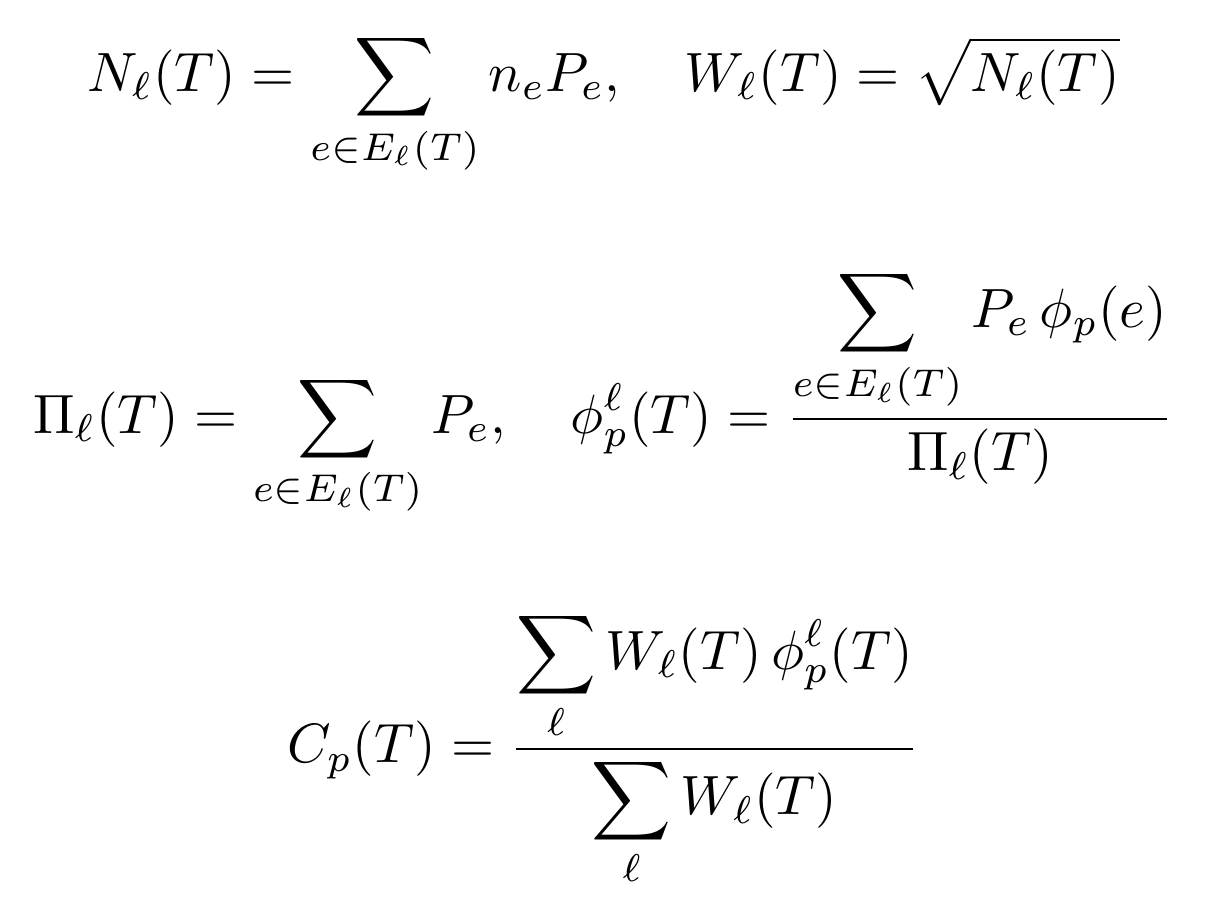
\includegraphics[width=0.9\linewidth]{images/formula_cp.png}
\end{center}


\textbf{階層内の合成}(都知事選と府知事選など、同じ種類の選挙をする自治体間の選挙)を考えます。人口$P_e$の加重平均$\phi_p^\ell(T)$を使います。$\phi_p^\ell(T)$は、政党$p$を代表(議員・首長)に選んだ人口の割合です。
この加重は、2つの町が合併しても合併前後で政党$p$が代表する人口の総和が変わりません。

\textbf{階層をまたぐ合成}(知事1人と議員1議席のように、単純には足し合わせられない異なる種類の代表を釣り合わせる場面)の重みには「ペンローズの平方根則」を援用しています。具体的には、当選者を全員1つの議事堂に集めて多数決させる状況を考え、代表者1人あたりの代表人口の平方根を重みとして足し合わせると$N_\ell(T)$の平方根$W_\ell(T)$という形が導けます(詳細は\href{https://github.com/hiromichikimura-lang/seiryoku-shisu/blob/master/design_document.pdf}{設計文書}を参照)。

集計期間を直近12か月の後方ウィンドウにしているのは、統一地方選のように選挙が特定の月に集中する季節性を、どの時点で切っても機械的にキャンセルできるからです。単月だけで集計すると、選挙が1件しか無い月とその月にたまたま無所属ばかり当選した月とで指数が極端に振れてしまいます。

なお、単純な政党比較は、以下のような慣行の違いがあるため困難です。
\begin{itemize}
\item \textbf{自民党系候補}: 地方議会選挙で党名を出さず無所属で出馬することが多い。
\item \textbf{共産党}: ほぼ必ず党名を出す。
\end{itemize}
一方、\textbf{同じ政党の値が時間とともにどう動いたか}は意味を持ちます。
推薦・支持政党データである程度は補正可能ですが、直近の公開遅れ(後述)で補正しきれない分が残ります。

個別に追跡する政党は、政党助成法上の「政党要件」(国会議員5人以上、または直近の国政選挙で得票率2\%以上)を満たす政党だけです。それ以外は無所属とまとめて扱います。

\section*{現在の指数の値(2026年8月時点)}

$C_p(T)$は前月以前と比較してこそ意味を持つ指標なので、遡れる限界(地方自治総合研究所の推薦・支持データが2018年版まで)である2018年1月〜2026年8月の全期間(104か月)を月次で再構成しています。

図\ref{fig:main}は、政党ごとに高さを正規化した党勢指数の推移(上段)、選挙の種類ごとの重みシェアの推移(中段)、首相の在任期間(下段)を並べたグラフです。上段は政党間の絶対水準を比べる意図はなく、複数の政党が同じ時期にどう動いたかを読み取るためのものです。

\begin{figure}[h]
\centering
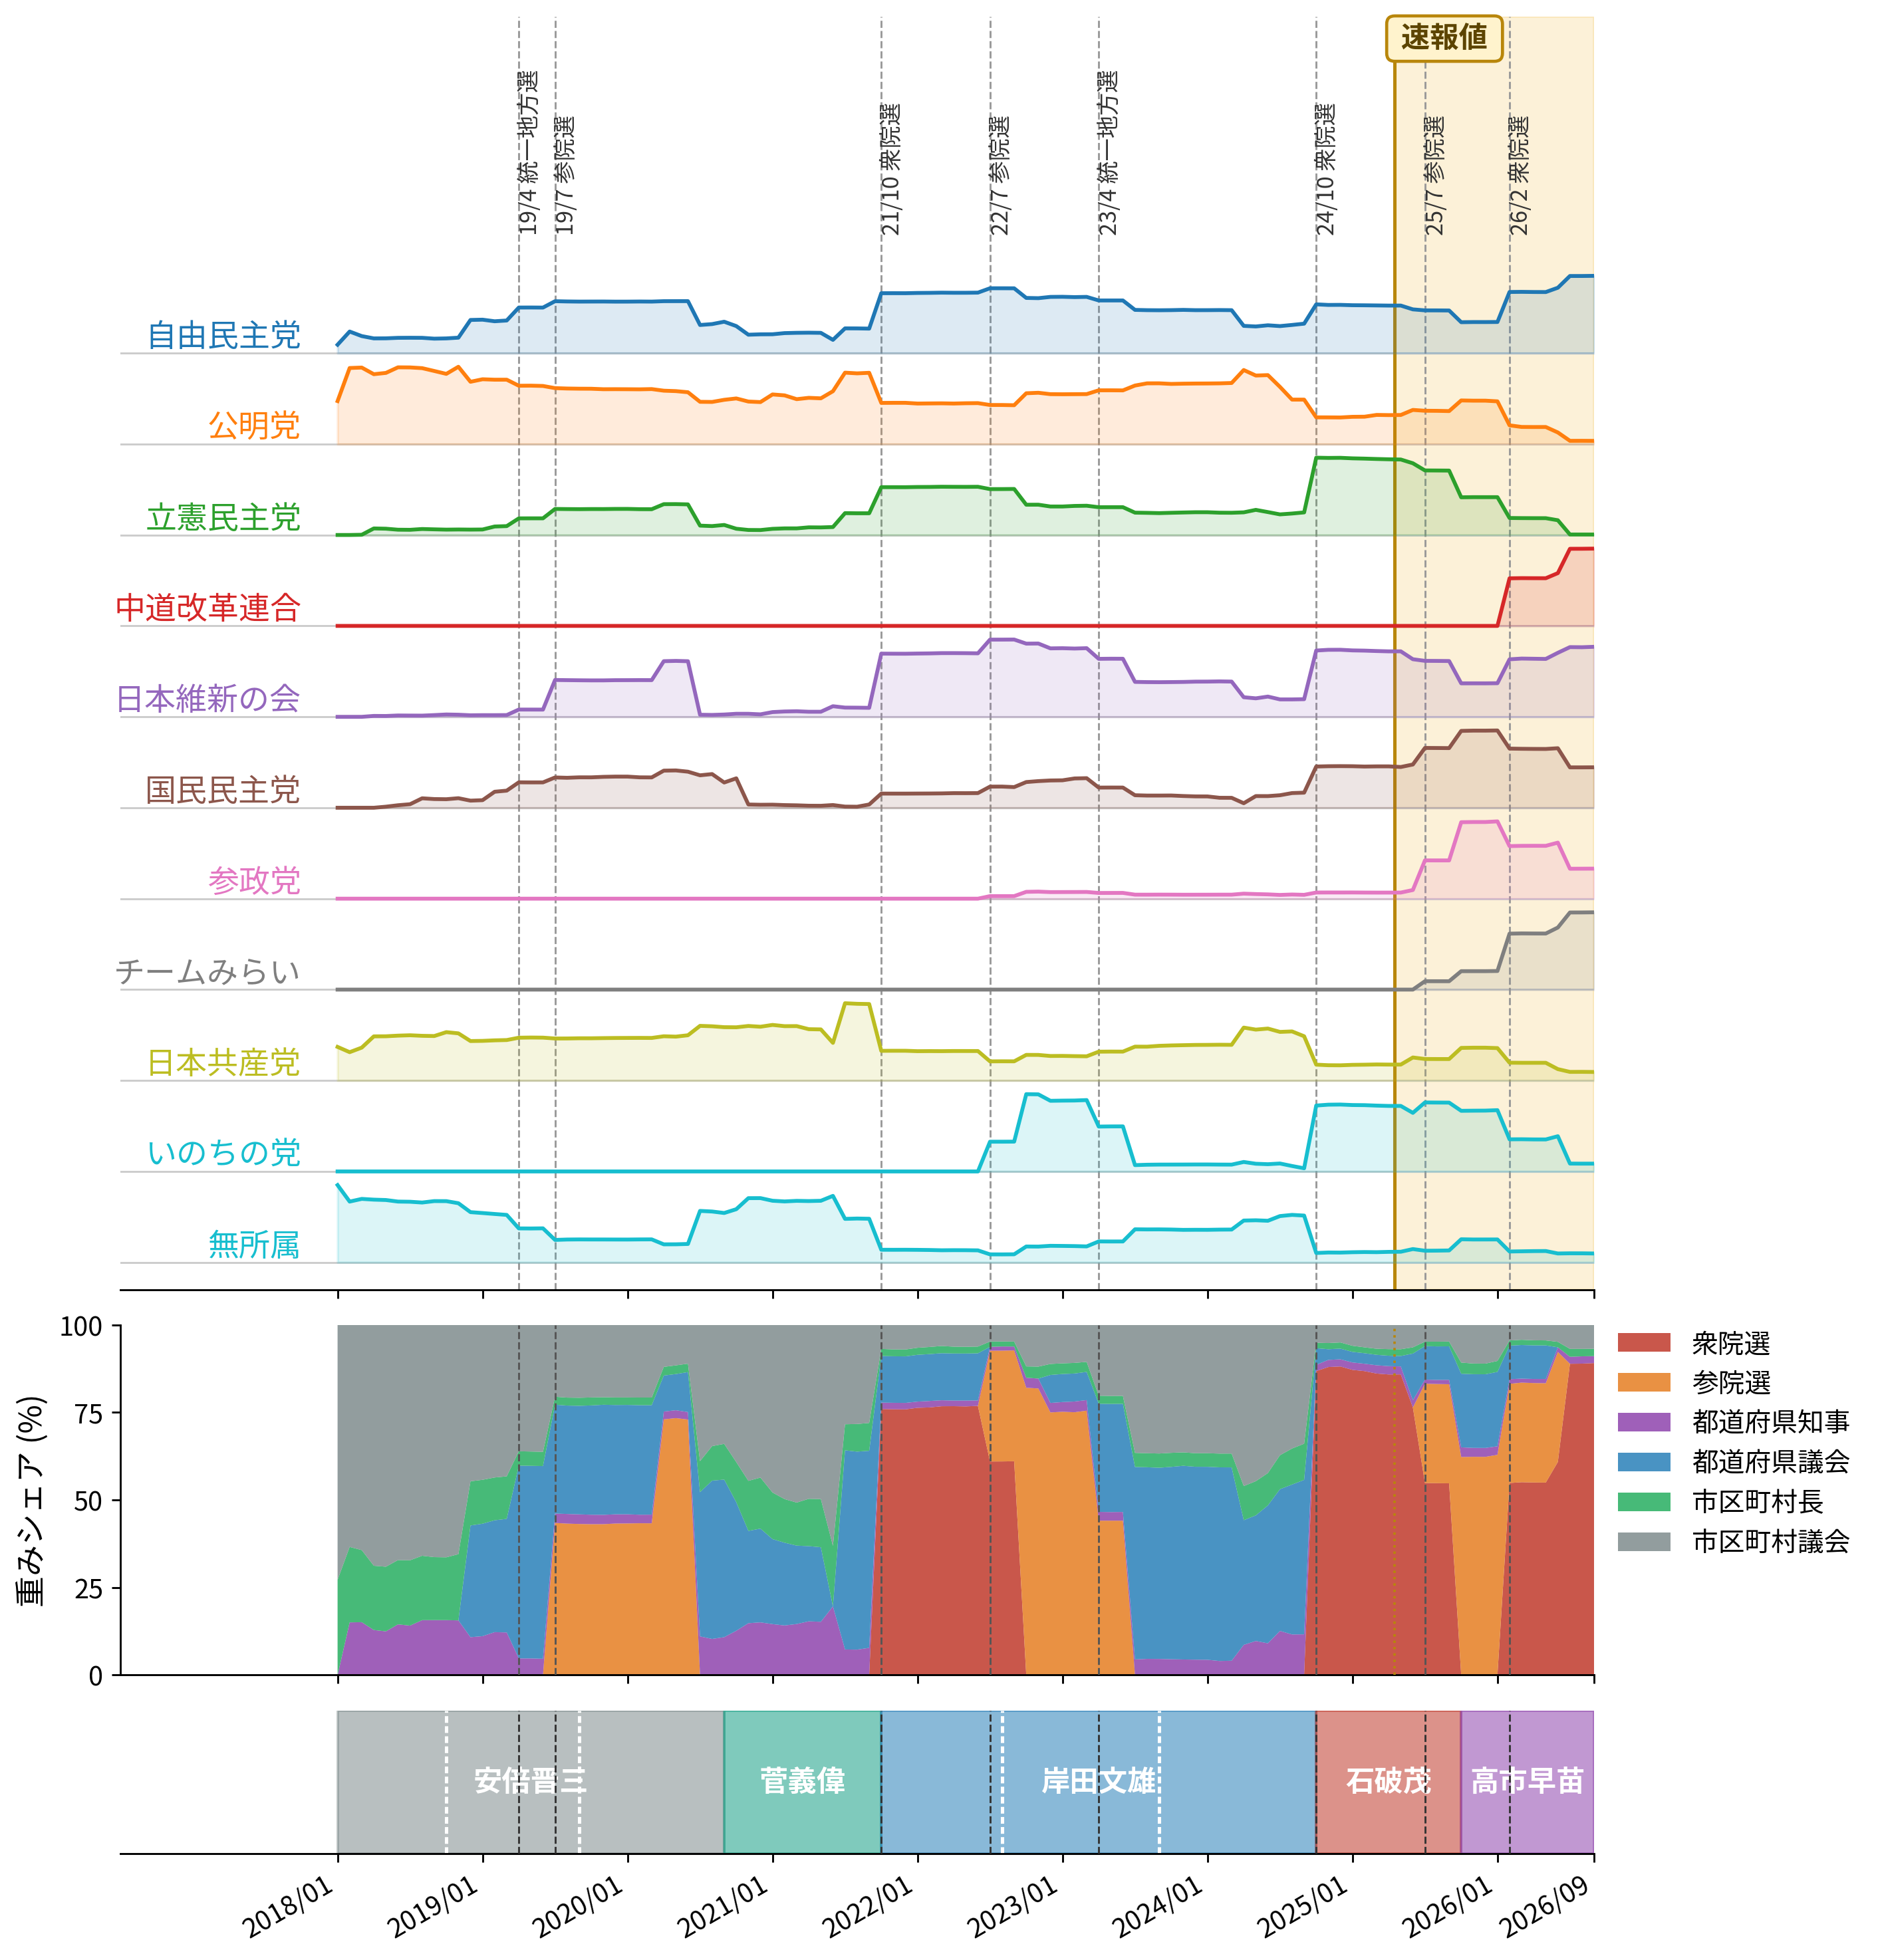
\includegraphics[width=0.95\textwidth]{images/cp_and_level_share.png}
\caption{党勢指数の政党別推移(上段)・選挙の種類ごとの重みの内訳(中段)・首相の在任期間(下段)}
\label{fig:main}
\end{figure}

無所属は直近数か月ぶんのデータ公開に構造的な遅れがあり、地方議会の多さもあって2026年9月時点で素の値は48.0\%に達します。上段のグラフは無所属を除いて正規化した値です。

首長の推薦・支持データ(地方自治総合研究所「全国首長名簿」)の最新版は2024年5月1日〜2025年4月30日の選挙までしか収録していないため、2025年5月以降を含む12か月ウィンドウは\textbf{速報値}として黄色く塗り、それより前を\textbf{確定値}としています。新しい年版が公開され次第、全期間を再計算します。

上段を貫くのこぎり状の動きは、一斉改選される選挙(国政選挙・都道府県議会)が12か月ウィンドウに入るたびに指数が振れ、12か月後に抜けると反動で戻るという機械的な挙動です。個別の山谷はそれぞれ実際の選挙で説明できます。

図\ref{fig:main}の中段を見ると、選挙の種類によって3つの挙動に分かれます。

\begin{itemize}
\item \textbf{市区町村議会}: 全期間を通じて27.9\%を下回らず、指数の基盤として常に一定の割合を保ちます。
\item \textbf{衆院選・参院選・都道府県議会}: 一斉改選の月の前後だけ急激に割合が高まり、それ以外はゼロに近づきます。
\item \textbf{都道府県知事・市区町村長}: 任期が自治体ごとにばらけているため、中間的な挙動を示します。
\end{itemize}

特定の選挙の種類が指数を単独で支配し続ける期間は存在しません。

図\ref{fig:main}の下段は首相の在任期間です。色の変わり目が首相交代、同じ色の帯の中にある白い破線が内閣改造(政権交代を伴わないもの)を示します。

\begin{itemize}
\item \textbf{首相交代(色の変わり目)}: 2020年9月・菅義偉、2021年10月・岸田文雄、2024年10月・石破茂、2025年10月・高市早苗。
\item \textbf{内閣改造(白い破線)}: 2018年10月・2019年9月の安倍改造内閣、2022年8月・2023年9月の岸田改造内閣。
\end{itemize}

首相交代はいずれも衆院選と同時期か選挙結果を受けた指名によるもので上段・中段の急変時期と重なる一方、内閣改造の時期には目立った変動が無く、選挙結果が指数を動かしていることの傍証です。

\textbf{2024年10月・衆院選}: 自民党が約32\%→39\%に急伸する一方、公明党は約29\%→12\%に急落(公明党代表の落選を含む苦戦が実際に報じられています)。ただしこの急伸は自民党自身の躍進ではありません。実際の議席は259から191へ減っており、野党票の分散や一部政党の追跡対象外化により、追跡対象政党どうしの相対シェアで自民党が押し上げられただけです。指数特有の見え方の一例です。

\subsection*{予測とサプライズについて}

第0回のうちに、今後の月次記事で「予測」欄を書くための裏付けを示します。統計的な検定の詳細はいずれも\href{https://github.com/hiromichikimura-lang/seiryoku-shisu/blob/master/design_document.pdf}{設計文書}に記載しています。

バックテストの対象は、安定した時系列を持つ6党(自由民主党・公明党・立憲民主党・日本維新の会・国民民主党・日本共産党)に絞りました。対象外の政党とその理由は次の通りです(いずれもデータが積み上がれば再検証します)。

\begin{itemize}
\item \textbf{中道改革連合・チームみらい}: 2026年2月結成で履歴不足。
\item \textbf{参政党}: 履歴はあるが国政選挙が絡む月が2件のみ。
\item \textbf{いのちの党}: 政党要件を満たしたり失ったりを繰り返し、時系列が不安定。
\end{itemize}

比較したのは次の3通りの予測手法です。

\begin{itemize}
\item \textbf{ゼロ予測}: 前月から変化なしと予測。
\item \textbf{モメンタム予測}: 前月の差分をそのまま継続すると予測。
\item \textbf{TimesFM-3}: Google Researchが2026年8月に公開した時系列予測モデルで、国政選挙のような既知の将来イベントを条件(covariate)として与えられる。
\end{itemize}

国政選挙が絡まない平常月では、ゼロ予測が最も当たり、モメンタム・TimesFM-3はむしろ悪化しました。方向的中率も52.9\%とコイン投げ水準で、ドリフトも自己相関も無く、$C_p(T)$の動きはランダムウォークで近似するのが妥当です。

国政選挙が絡む月(選挙月とその12か月後の窓抜け月、計11か月)では対照的に、TimesFM-3が明確な方向感を示しました。6党をプールした順位相関は0.50で、モメンタムの0.12を上回ります。ただし政党ごとの個別検定は標本数n=11では非力で、多重比較を補正すると日本共産党しか有意性が残りません(政党別の詳しい数値・検定手法は\href{https://github.com/hiromichikimura-lang/seiryoku-shisu/blob/master/design_document.pdf}{設計文書}に記載しています)。

\textbf{採用ルール}: 個別の有意性で線引きすると事後的な選別になるため、プールした検定結果を優先し、国政選挙が絡む月は6党全てにTimesFM-3を使い、それ以外(平常月・対象外政党)は予測を出しません(暫定的な区切りです)。

採用ルールの予測値が実測と大きく乖離したケースには、理由が分かるものと分からないものがありました。

\begin{itemize}
\item \textbf{理由が分かるもの(2024年10月、公明党・立憲民主党)}: 政治資金問題への批判票が立憲民主党に集まり(実測$+16.4$pt、予測$+1.5$pt)、公明党は代表の落選を含む苦戦をしたことが実際に報じられている月でした(実測$-17.4$pt、予測$-6.4$pt)。TimesFM-3は方向は捉えたものの、動きの大きさまでは予測できませんでした。
\end{itemize}

他の事例(符号が逆転した2026年7月の自民党など)は\href{https://github.com/hiromichikimura-lang/seiryoku-shisu/blob/master/design_document.pdf}{設計文書}にまとめています。

実際の値との差分(サプライズ)は毎月確認し、大きな乖離は単月の生データまで裏取りしてから記事にします。来月(2026年10月)は国政選挙が無いため、採用ルールに従って予測は出しません。

\subsection*{おまけ: 「地方選は国政選挙の前哨戦」は本当か}

政治報道でよく言われる「統一地方選のような地方選挙は、次の国政選挙の前哨戦になる」という言説を検証してみました。国会の選挙(衆院選・参院選)だけを除いた「地方選挙限定の$C_p(t)$」を作り、実際にあった国政選挙の結果と突き合わせています。

\textbf{地方の勢いの変化の方向と、国政選挙での議席の増減方向を比べました。} 衆院選・参院選それぞれ連続する2回の組(計4組)について、政党ごとに方向が一致するかを見たところ、立憲民主党・国民民主党・日本共産党の3党は4組\textbf{全て}で方向が一致し、日本維新の会は4組\textbf{全て}で方向が逆でした。6党のうち4党がこれほど極端に揃う確率は、方向がランダムだとすると0.3\%程度で、単なる偶然にしては起こりにくい結果です(全党をまとめた一致率は70\%どまりで、この党ごとの偏りは隠れてしまいます)。今後、国政選挙が行われるたびにこの表を更新し、パターンが崩れないか検証を続けます。

\textbf{逆方向、つまり国政選挙の結果がその後の地方選挙の動きに持ち越されるかも確認しました。} 国政選挙があった月の直後1か月の実測差分は、他の平常月と比べて平均に有意差が無く、国政選挙月自体の実測差分と翌月の実測差分にも相関はありませんでした。少なくとも1か月先までは、国政選挙の勢いが地方選挙側に持ち越される効果は見つかりませんでした。

\textbf{ここまでを総合すると、地方選挙は国政選挙の縮図ではなく、ほぼ独立に動いているという描像になります。} 国政選挙が絡まない月の$C_p(T)$はランダムウォークに近く、国政選挙の結果が翌月以降の地方選挙に持ち越された形跡もありません。唯一残るのは逆方向、つまり地方選挙の勢いの変化の\textbf{方向}が次の国政選挙の結果の方向とある程度対応するという弱い証拠で、これも大きさの対応までは確認できていません。「地方選は国政選挙の前哨戦」という話は、方向に限れば部分的に裏付けられます。

\section*{今後について}

更新は月1回を目安にします。あくまで個人の趣味の定点観測です。次回以降は次の4本立てで淡々と続けます。

\begin{enumerate}[nosep]
\item 直近月の選挙概況
\item 前回予測を出していれば、その答え合わせ
\item 大きな動きがあれば実際にサプライズだったのか裏取り
\item 次の月が国政選挙に絡む場合のみ、予測
  \begin{itemize}[nosep]
  \item \textbf{主予測}: 国政選挙が絡む月はバックテスト対象の6党全てにTimesFM-3を使用。
  \item \textbf{「地方選は国政選挙の前哨戦」仮説の検証}: 次の国政選挙のたびに検証表を更新。
  \end{itemize}
\end{enumerate}

個別の地方選挙結果の予測のような対象は増やしません。

\section*{データソース}

衆参の議席・地方議会の議席・首長の選挙結果・推薦支持政党データをどこからどう取得しているかは\href{https://github.com/hiromichikimura-lang/seiryoku-shisu/blob/master/design_document.pdf}{設計文書}としてまとめてあり、算出コードとあわせて\href{https://github.com/hiromichikimura-lang/seiryoku-shisu}{GitHub}で公開しています。誰でも検証できる形にしています。

\section*{著作権について}

算出コードはMITライセンスで公開し、自由に使ってもらって構いません。ただしこの記事や設計文書など、文章そのものの著作権は放棄していません。

\section*{AI活用について}

指数の設計・データソース調査・実装には、AI(Claude)を活用しています。


\end{document}
